\documentclass[a4paper,12pt]{article}
\usepackage{czech}
\usepackage[utf8]{inputenc}
\usepackage{a4wide}
\usepackage[dvipdfm]{graphicx}
\usepackage{graphics}
\usepackage{indentfirst}
\usepackage{fancyhdr}
\usepackage{setspace}
\usepackage{amsmath}
\usepackage{amssymb}
\usepackage{epsfig}

%%\usepackage{nopageno}
%%\usepackage{txfonts}
\usepackage[usenames]{color}

\begin{document}
%\input{../../titulka.sty}
%\praktikum{Praktikum II - Elektřina a magnetizmus}
%\uloha{6}
%\nazev{Měření účiníku}
%\pracant{Lukáš Beran}
%\skupina{13}
%\denprace{21. 11. 2011}

\section{Úkol}
\noindent
\begin{enumerate}
    \item Změřte účiník:
        \begin{enumerate}
            \item rezistoru,
            \item kondenzátoru ($C$ = 10 $\mu$F)
            \item cívky. 
        \end{enumerate}
    Určete chybu měření. Diskutujte shodu výsledků s teoretickými hodnotami pro ideální prvky. Pro cívku vypočtěte indukčnost a odpor v sériovém a paralelním náhradním zapojení.
    \item Změřte účiník sériového a paralelního zapojení rezistoru a kondenzátoru ( $C$ = 1; 2; 5; 10 $\mu$F). Z naměřených hodnot stanovte odpor rezistoru. Určete chyby měření a rozhodněte, které z obou zapojení je v daném případě vhodnější pro stanovení odporu.
    \item Změřte závislost proudu a výkonu na velikosti kapacity zařazené do sériového RLC obvodu.
    \item Výsledky úkolu 3. zpracujte graficky, v závislosti na zařazené kapacitě vyneste účiník, fázový posuv napětí vůči proudu a výkon. 
\end{enumerate}

\section{Teorie}

\subsection{Účiník}
Výkon střídavého proudu za určitý čas $T$ je definován
\begin{eqnarray}
P=\frac{1}{T}\int^T_0u(t)i(t)\mbox{d}t,
\end{eqnarray}
kde $u$ a $i$ jsou okamžité hodnoty proudu a napětí. Pro sinusový průběh proudu, kde $\varphi$ je fázový rozdíl napětí vůči proudu získáme integrací
\begin{eqnarray}
P=\frac{U_0I_0}{2}\cos\varphi,
\label{P1}
\end{eqnarray}
což můžeme pro efektivní hodnoty upravit na
\begin{eqnarray}
P=UI\cos\varphi.
\label{P2}
\end{eqnarray}

Účiník je $\cos\varphi$ z rovnic \ref{P1} a \ref{P2}, z kterých ho snadno vypočítáme.

\subsection{Resistance, kapacitance a induktance}
Resistance nijak neovlivňuje velikost účiníku. V obvodu, ve kterém je pouze odpor je účiník roven jedné. Pokud je v obvodu poze kondenzátor, vzniká fázový posun napětí $\varphi$, který 
je v ideálním případě roven $\frac{-\pi}{2}$. Podobná situace nastane u cívky, kdy je $\varphi=\frac{\pi}{2}$. V obou případech je účiník roven nule.

Při zapojení více prvků do série pro fázový posuni napětí vůči proudu platí
\begin{eqnarray}
\varphi=\arctan\frac{\omega L-\frac{1}{\omega C}}{R},
\end{eqnarray}
kde $L$ je indukčnost, $C$ kapacita a $R$ celkový odpor obvodu. Při paralelním zapojení platí 
pro fázový posun proudu vůči napětí $\varphi'$
\begin{eqnarray}
\varphi'=\arctan\left(\omega RC-\frac{R}{\omega L}\right).
\end{eqnarray}

\subsection{Výpočet $L$, $R$ a $C$}
Při zapojení cívky a odporu dá snadno vypočítat velikosti indukčnisti a odporu. Dle \cite{text} pro sériové zapojení platí
\begin{eqnarray}
R_S=\frac{U}{I}\frac{1}{\sqrt{1+\tan^2\varphi}} \label{LRS}\\ 
L_S=\frac{U}{\omega I}\sqrt{\frac{\tan^2\varphi}{1+\tan^2\varphi}}
\label{LLS}
\end{eqnarray}
a pro paralení platí
platí
\begin{eqnarray}
R_P=\frac{U}{I}\sqrt{1+\tan^2\varphi}\\
\label{LRP}
L_P=\frac{U}{\omega I}\sqrt{\frac{1+\tan^2\varphi}{\tan^2\varphi}}
\label{LLP}
\end{eqnarray}

Podobné vzahy platí i pro zapojení kondenzátoru a odporu. Konkrétní rovnice jsou
\begin{eqnarray}
R_S=\frac{U}{I}\frac{1}{\sqrt{1+\tan^2\varphi}}
\label{CRS}\\
C_S=\frac{U}{\omega I}\sqrt{\frac{1+\tan^2\varphi}{\tan^2\varphi}}
\label{CCS}\\
R_P=\frac{U}{I}\sqrt{1+\tan^2\varphi}
\label{CRP}\\
C_P=\frac{U}{\omega I}\sqrt{\frac{\tan^2\varphi}{1+\tan^2\varphi}}
\label{CLP}
\end{eqnarray}

\subsection{Chyby}
Při měření byla použita jak analogová, tak digitálí zařízení. Pro chybu anologových musíme 
znát jejich třídu přesnosti. V tomto případě se jednalo o ampérmetri resp. watmetr, který měl třídu 
přesnoti 1.5 resp. 0.2. Velikost aboslutní chyby získáme
\begin{eqnarray}
\sigma=1.5\frac{R}{100},
\end{eqnarray}
kde $R$ je rozsah ampérmetru resp. watmetru.

Digitální přístroje mají svou procentuální chybu naměřené hodnoty, ke které se přičte jistá hodnota v řádu poslední číslice na dipleji. Voltmetr měl 
konkrétně chybu $\pm 2.5\% \pm 10d$.

\section{Měření}
\begin{figure}
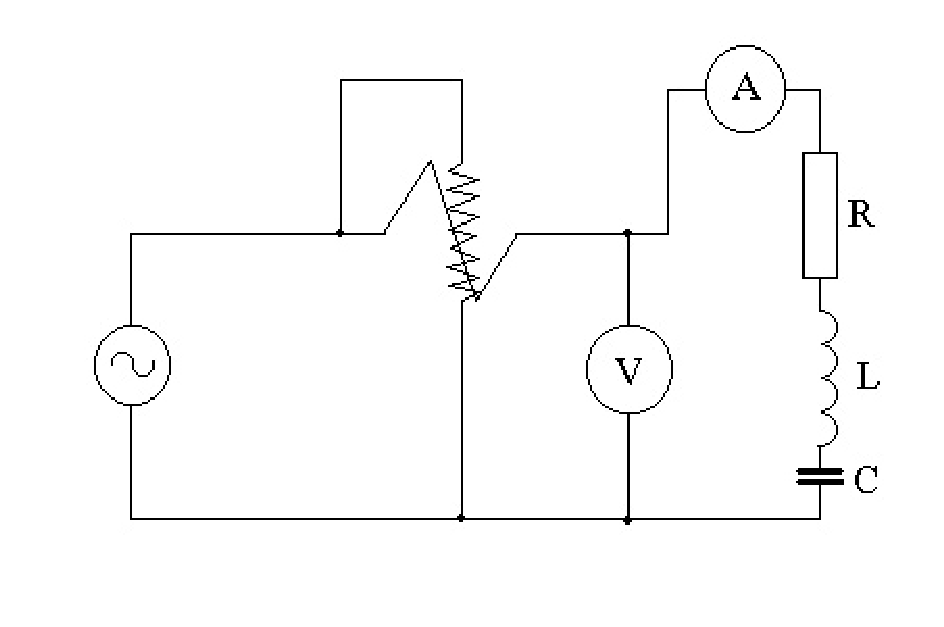
\includegraphics{sch1.eps}
\caption{Schéma měření}
\label{sch1}
\end{figure}

\subsection{Účiník odporu, cívky a kondenzátoru}
Zapojil jsem měřící přístroje dle obrázku \ref{sch1} a postupně jsem zapojoval jednotlivé součástky. Následně jsem zapojil cívku s odporem, a 
to jak sériově, tak paralelně. Naměřené hodnoty se spočteným účiníkem jsou v tabulce \ref{TUk1}. 
Z posledních dvou jsem vypočetl odpor a indukčnost v náhradním zapojení
\begin{eqnarray}
R_s&=&(1.6\pm0.2) \mbox{k}\Omega \\
L_s&=&(60\pm6) \mu\mbox{H}\\
R_p&=&(1.0\pm0.1) \mbox{k}\Omega \\
L_s&=&(3.6\pm0.4)\mbox{H}
\end{eqnarray}

\begin{table}
$$
\begin{array}{|c|c|c|c||c|}
\hline
&   U/\mbox{V}& I/\mbox{mA}&    P/\mbox{W}& \cos\varphi \\ \hline
R&  51 \pm 1&   44\pm 2&    2.00\pm 0.07&   0.89 \pm 0.09 \\ \hline
L&  51 \pm 1&   29\pm 2&    0.50\pm 0.07&   0.33 \pm 0.08  \\ \hline
C&  51 \pm 1&   140\pm 5&   0.00\pm 0.07&   0.00 \pm 0.08 \\ \hline
RL s.&  51\pm1& 21.0\pm 0.5&    0.70 \pm 0.07&  0.65\pm 0.09\\ \hline
RL p.&  51\pm1& 67\pm2&     2.55 \pm 0.07&  0.75\pm 0.06\\ \hline
\end{array}
$$
\caption{Hodnoty naměřné v úkolu 1.}
\label{TUk1}
\end{table}

\subsection{Odpor a kondenzátor}
Pro sériové a paralelní zapojení odporu a kondenzátoru jsem měřil charakteristiky s různými kapacitami. Naměřené hodnoty jsou v tabulkách \ref{RCs} a \ref{RCp}. 
Tato zapojení jsem také o něco hustěji proměřil digitálním měřákem, který rovnou ukazoval i velikost účiníku. Výsledky tohoto měření jsou v tabulkách \ref{RCs2} a \ref{RCp2} spolu 
s dopočteným odporem.

\begin{table}
$$
\begin{array}{|c|c|c|c|c||c|}
\hline
C/\mu\mbox{F}&  U/\mbox{V}& I/\mbox{mA}&    P/\mbox{W}& \cos\varphi&    R/\Omega \\ \hline
1&  51\pm1& 53\pm2& 2.00\pm0.07&    0.74\pm0.07&    710\pm 70 \\ \hline
2&  51\pm1& 61\pm2& 2.05\pm 0.07&   0.66\pm0.06&    550\pm 50 \\ \hline
5&  51\pm1& 100\pm5&    2.10\pm 0.07&   0.41\pm0.04&    210\pm 20 \\ \hline
10& 51\pm1& 160\pm5&    2.10\pm 0.07&   0.26\pm0.02&    80\pm 8 \\ \hline
\end{array}
$$
\caption{Sériové zapojení kondenzátoru a odporu}
\label{RCs}
\end{table}

\begin{table}
$$
\begin{array}{|c|c|c|c|c||c|}
\hline
C/\mu\mbox{F}&  U/\mbox{V}& I/\mbox{mA}&    P/\mbox{W}& \cos\varphi& R/\Omega \\ \hline
1&  51\pm1& 15\pm0.5& 0.20\pm0.07&    0.3\pm0.1&    10 000\pm 1000 \\ \hline
2&  51\pm1& 27.5\pm0.5& 0.60\pm 0.07&   0.43\pm0.07&    4000\pm 400 \\ \hline
5&  51\pm1& 44\pm2&    1.50\pm 0.07&   0.67\pm0.07& 1700\pm 200 \\ \hline
10& 51\pm1& 49\pm2&    1.90\pm 0.07&   0.76\pm0.07& 1400\pm 100 \\ \hline
\end{array}
$$
\caption{Paralelní zapojení kondenzátoru a odporu}
\label{RCp}
\end{table}

\begin{table}
$$
\begin{array}{|c|c|c|c|c|}
\hline
C/\mu\mbox{F}&  U/\mbox{V}& I/\mbox{mA}&    P/\mbox{W}& \cos\varphi \\ \hline
1&  50.9\pm0.7& 15\pm5& 0.24\pm0.01&    0.31\pm0.04 \\ \hline
2&  50.9\pm0.7& 27\pm5& 0.75\pm0.02&    0.54\pm0.04 \\ \hline
3&  50.7\pm0.7& 35\pm5& 1.22\pm0.02&    0.69\pm0.04 \\ \hline
4&  50.9\pm0.7& 40\pm5& 1.59\pm0.02&    0.79\pm0.05 \\ \hline
5&  50.9\pm0.7& 43\pm5& 1.86\pm0.03&    0.85\pm0.05 \\ \hline
6&  50.9\pm0.7& 45\pm5& 2.04\pm0.03&    0.89\pm0.05 \\ \hline
7&  50.9\pm0.7& 46\pm5& 2.15\pm0.03&    0.91\pm0.05 \\ \hline
8&  50.9\pm0.7& 47\pm5& 2.23\pm 0.03&   0.93\pm0.05 \\ \hline
9&  50.8\pm0.7& 48\pm5&    2.30\pm 0.03&   0.95\pm0.05 \\ \hline
10& 50.9\pm0.7& 48\pm5&    2.35\pm 0.03&   0.96\pm0.05 \\ \hline
\end{array}
$$
\caption{Sériové zapojení kondenzátoru a odporu měřeno digitální měřákem.}
\label{RCs2}
\end{table}

\begin{table}
$$
\begin{array}{|c|c|c|c|c|}
\hline
C/\mu\mbox{F}&  U/\mbox{V}& I/\mbox{mA}&    P/\mbox{W}& \cos\varphi \\ \hline
1&  50.7\pm0.7& 54\pm5& 2.58\pm0.03&    0.94\pm0.05 \\ \hline
2&  50.7\pm0.7& 61\pm5& 2.58\pm0.03&    0.84\pm0.05 \\ \hline
3&  50.7\pm0.7& 71\pm5& 2.58\pm0.03&    0.72\pm0.04 \\ \hline
4&  50.7\pm0.7& 83\pm5& 2.58\pm0.03&    0.62\pm0.04 \\ \hline
5&  50.8\pm0.7& 96\pm5& 2.58\pm0.03&    0.53\pm0.04 \\ \hline
6&  50.8\pm0.7& 110\pm5& 2.58\pm0.03&    0.46\pm0.04 \\ \hline
7&  50.8\pm0.7& 125\pm6& 2.58\pm0.03&    0.41\pm0.04 \\ \hline
8&  50.8\pm0.7& 140\pm6& 2.59\pm 0.03&   0.36\pm0.04 \\ \hline
9&  50.8\pm0.7& 155\pm6&    2.59\pm 0.03&   0.33\pm0.04 \\ \hline
10& 50.8\pm0.7& 171\pm6&    2.59\pm 0.03&   0.30\pm0.04 \\ \hline
\end{array}
$$
\caption{Paralelně zapojení kondenzátoru a odporu měřeno digitální měřákem.}
\label{RCp2}
\end{table}

\subsection{Sériový RLC obvod}
Do série jsem zapojil rezistor, cívku a kondenzátor a měřil jsem závislost proudu a výkonu na kapacitě. Následně jsem dopočítal účiník a fázový posun napětí vůči proudu. 
Výsledky měření jsou v tabulce \ref{TUk3} zaneseny do grafu na obrázku \ref{g1}. Pro názornost jsou data proložené křivkou.
\begin{table}
$$
\begin{array}{|c|c|c|c|c|c|}
\hline
C/\mu\mbox{F}&  U/\mbox{V}& I/\mbox{mA}&    P/\mbox{W}& \cos\varphi&    \varphi\\ \hline
0.1&51\pm 1&1.6\pm 0.2&0.00\pm 0.07&0.0\pm 0.2&2\pm1\\ \hline
0.2&51\pm 1&3.3\pm 0.2&0.00\pm 0.07&0.0\pm 0.2&2\pm1\\ \hline
0.3&51\pm 1&5.1\pm 0.2&0.00\pm 0.07&0.0\pm 0.2&2\pm1\\ \hline
0.4&51\pm 1&6.9\pm 0.2&0.10\pm 0.07&0.2\pm 0.2&1\pm1\\ \hline
0.5&51\pm 1&8.8\pm 0.2&0.10\pm 0.07&0.2\pm 0.2&1\pm1\\ \hline
0.6&51\pm 1&11.0\pm 0.5&0.10\pm 0.07&0.2\pm 0.1&1.4\pm1\\ \hline
0.7&51\pm 1&13.5\pm 0.5&0.20\pm 0.07&0.3\pm 0.1&1.3\pm0.5\\ \hline
0.8&51\pm 1&16.0\pm 0.5&0.30\pm 0.07&0.47\pm 0.1&1.2\pm0.3\\ \hline
0.9&51\pm 1&18.5\pm 0.5&0.40\pm 0.07&0.42\pm 0.09&1.1\pm0.3\\ \hline
1.0&51\pm 1&20.5\pm 0.5&0.50\pm 0.07&0.48\pm 0.09&1.1\pm0.2\\ \hline
1.1&51\pm 1&23.0\pm 0.5&0.70\pm 0.07&0.60\pm 0.08&0.9\pm0.1\\ \hline
1.2&51\pm 1&24.5\pm 0.5&0.80\pm 0.07&0.64\pm 0.08&0.9\pm0.1\\ \hline
1.3&51\pm 1&26.5\pm 0.5&0.90\pm 0.07&0.67\pm 0.08&0.8\pm0.1\\ \hline
1.4&51\pm 1&27.5\pm 0.5&1.00\pm 0.07&0.71\pm 0.08&0.78\pm0.08\\ \hline
1.5&51\pm 1&28.5\pm 0.5&1.10\pm 0.07&0.76\pm 0.08&0.71\pm0.07\\ \hline
1.6&51\pm 1&29.0\pm 0.5&1.10\pm 0.07&0.74\pm 0.07&0.73\pm0.07\\ \hline
1.7&51\pm 1&29.5\pm 0.5&1.20\pm 0.07&0.80\pm 0.08&0.65\pm0.06\\ \hline
1.8&51\pm 1&30.0\pm 0.5&1.20\pm 0.07&0.78\pm 0.07&0.67\pm0.06\\ \hline
1.9&51\pm 1&30.0\pm 0.5&1.20\pm 0.07&0.78\pm 0.07&0.67\pm0.06\\ \hline
2.0&51\pm 1&30.0\pm 0.5&1.20\pm 0.07&0.78\pm 0.07&0.67\pm0.06\\ \hline
2.5&51\pm 1&29.5\pm 0.5&1.20\pm 0.07&0.80\pm 0.08&0.65\pm0.06\\ \hline
3.0&51\pm 1&29.0\pm 0.5&1.10\pm 0.07&0.74\pm 0.07&0.73\pm0.07\\ \hline
3.5&51\pm 1&28.5\pm 0.5&1.00\pm 0.07&0.69\pm 0.07&0.81\pm0.09\\ \hline
4.0&51\pm 1&27.5\pm 0.5&1.00\pm 0.07&0.71\pm 0.08&0.78\pm0.08\\ \hline
4.5&51\pm 1&27.5\pm 0.5&1.00\pm 0.07&0.71\pm 0.08&0.78\pm0.08\\ \hline
5.0&51\pm 1&27.0\pm 0.5&1.00\pm 0.07&0.73\pm 0.08&0.76\pm0.08\\ \hline
5.5&51\pm 1&26.5\pm 0.5&0.90\pm 0.07&0.67\pm 0.08&0.8\pm0.1\\ \hline
6.0&51\pm 1&26.5\pm 0.5&0.90\pm 0.07&0.67\pm 0.08&0.8\pm0.1\\ \hline
6.5&51\pm 1&26.5\pm 0.5&0.90\pm 0.07&0.67\pm 0.08&0.8\pm0.1\\ \hline
7.0&51\pm 1&26.0\pm 0.5&0.90\pm 0.07&0.68\pm 0.08&0.8\pm0.1\\ \hline
8.0&51\pm 1&25.5\pm 0.5&0.90\pm 0.07&0.69\pm 0.08&0.81\pm0.09\\ \hline
9.0&51\pm 1&25.5\pm 0.5&0.80\pm 0.07&0.62\pm 0.08&0.9\pm0.1\\ \hline
10.0&51\pm 1&25.5\pm 0.5&0.80\pm 0.07&0.62\pm 0.08&0.9\pm0.1\\ \hline
\end{array}
$$
\caption{Závislost výkonu, účiníku a fázového posunu napětí vůči proudu na kapacitě.}
\label{TUk3}
\end{table}

\begin{figure}
% GNUPLOT: LaTeX picture with Postscript
\begingroup
  \makeatletter
  \providecommand\color[2][]{%
    \GenericError{(gnuplot) \space\space\space\@spaces}{%
      Package color not loaded in conjunction with
      terminal option `colourtext'%
    }{See the gnuplot documentation for explanation.%
    }{Either use 'blacktext' in gnuplot or load the package
      color.sty in LaTeX.}%
    \renewcommand\color[2][]{}%
  }%
  \providecommand\includegraphics[2][]{%
    \GenericError{(gnuplot) \space\space\space\@spaces}{%
      Package graphicx or graphics not loaded%
    }{See the gnuplot documentation for explanation.%
    }{The gnuplot epslatex terminal needs graphicx.sty or graphics.sty.}%
    \renewcommand\includegraphics[2][]{}%
  }%
  \providecommand\rotatebox[2]{#2}%
  \@ifundefined{ifGPcolor}{%
    \newif\ifGPcolor
    \GPcolorfalse
  }{}%
  \@ifundefined{ifGPblacktext}{%
    \newif\ifGPblacktext
    \GPblacktexttrue
  }{}%
  % define a \g@addto@macro without @ in the name:
  \let\gplgaddtomacro\g@addto@macro
  % define empty templates for all commands taking text:
  \gdef\gplbacktext{}%
  \gdef\gplfronttext{}%
  \makeatother
  \ifGPblacktext
    % no textcolor at all
    \def\colorrgb#1{}%
    \def\colorgray#1{}%
  \else
    % gray or color?
    \ifGPcolor
      \def\colorrgb#1{\color[rgb]{#1}}%
      \def\colorgray#1{\color[gray]{#1}}%
      \expandafter\def\csname LTw\endcsname{\color{white}}%
      \expandafter\def\csname LTb\endcsname{\color{black}}%
      \expandafter\def\csname LTa\endcsname{\color{black}}%
      \expandafter\def\csname LT0\endcsname{\color[rgb]{1,0,0}}%
      \expandafter\def\csname LT1\endcsname{\color[rgb]{0,1,0}}%
      \expandafter\def\csname LT2\endcsname{\color[rgb]{0,0,1}}%
      \expandafter\def\csname LT3\endcsname{\color[rgb]{1,0,1}}%
      \expandafter\def\csname LT4\endcsname{\color[rgb]{0,1,1}}%
      \expandafter\def\csname LT5\endcsname{\color[rgb]{1,1,0}}%
      \expandafter\def\csname LT6\endcsname{\color[rgb]{0,0,0}}%
      \expandafter\def\csname LT7\endcsname{\color[rgb]{1,0.3,0}}%
      \expandafter\def\csname LT8\endcsname{\color[rgb]{0.5,0.5,0.5}}%
    \else
      % gray
      \def\colorrgb#1{\color{black}}%
      \def\colorgray#1{\color[gray]{#1}}%
      \expandafter\def\csname LTw\endcsname{\color{white}}%
      \expandafter\def\csname LTb\endcsname{\color{black}}%
      \expandafter\def\csname LTa\endcsname{\color{black}}%
      \expandafter\def\csname LT0\endcsname{\color{black}}%
      \expandafter\def\csname LT1\endcsname{\color{black}}%
      \expandafter\def\csname LT2\endcsname{\color{black}}%
      \expandafter\def\csname LT3\endcsname{\color{black}}%
      \expandafter\def\csname LT4\endcsname{\color{black}}%
      \expandafter\def\csname LT5\endcsname{\color{black}}%
      \expandafter\def\csname LT6\endcsname{\color{black}}%
      \expandafter\def\csname LT7\endcsname{\color{black}}%
      \expandafter\def\csname LT8\endcsname{\color{black}}%
    \fi
  \fi
  \setlength{\unitlength}{0.0500bp}%
  \begin{picture}(7200.00,5040.00)%
    \gplgaddtomacro\gplbacktext{%
      \csname LTb\endcsname%
      \put(1210,704){\makebox(0,0)[r]{\strut{} 700}}%
      \put(1210,1074){\makebox(0,0)[r]{\strut{} 800}}%
      \put(1210,1444){\makebox(0,0)[r]{\strut{} 900}}%
      \put(1210,1814){\makebox(0,0)[r]{\strut{} 1000}}%
      \put(1210,2184){\makebox(0,0)[r]{\strut{} 1100}}%
      \put(1210,2554){\makebox(0,0)[r]{\strut{} 1200}}%
      \put(1210,2925){\makebox(0,0)[r]{\strut{} 1300}}%
      \put(1210,3295){\makebox(0,0)[r]{\strut{} 1400}}%
      \put(1210,3665){\makebox(0,0)[r]{\strut{} 1500}}%
      \put(1210,4035){\makebox(0,0)[r]{\strut{} 1600}}%
      \put(1210,4405){\makebox(0,0)[r]{\strut{} 1700}}%
      \put(1210,4775){\makebox(0,0)[r]{\strut{} 1800}}%
      \put(1342,484){\makebox(0,0){\strut{} 0}}%
      \put(2263,484){\makebox(0,0){\strut{} 0.5}}%
      \put(3184,484){\makebox(0,0){\strut{} 1}}%
      \put(4105,484){\makebox(0,0){\strut{} 1.5}}%
      \put(5027,484){\makebox(0,0){\strut{} 2}}%
      \put(5948,484){\makebox(0,0){\strut{} 2.5}}%
      \put(6869,484){\makebox(0,0){\strut{} 3}}%
      \put(308,2739){\rotatebox{-270}{\makebox(0,0){\strut{}$h$/keV$\cdot$m$^{-1}$}}}%
      \put(4105,154){\makebox(0,0){\strut{}$x$/cm}}%
    }%
    \gplgaddtomacro\gplfronttext{%
    }%
    \gplbacktext
    \put(0,0){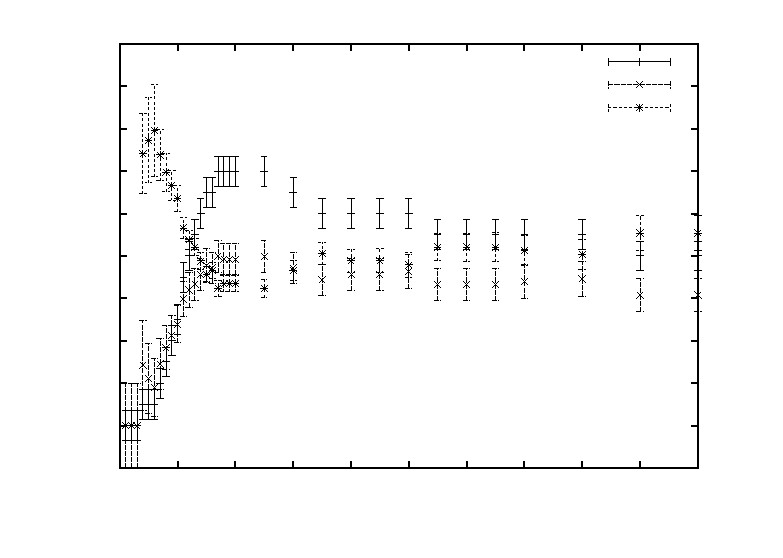
\includegraphics{g1}}%
    \gplfronttext
  \end{picture}%
\endgroup

\caption{Graf závislosti výkonu, účiníku a fázového posunu napětí vůči proudu na kapacitě.}
\label{g1}
\end{figure}

\section{Diskuze}
Při měření účiníku byla konečné chyba okolo 10 \%. To bylo způsobeno zejména vysokou relativní 
chybou na wattmetru. Ač bylo toto zařízení velice přesné, na chybě se výrazně podepsalo to, že 
jsem měřil ve spodní části stupnice. V tomto případě by pomohla změna rozsahu.

Jako nejideálnější prvek se jevil kondenzátor. Pouze u něj odpovídala velikost účiníku teorii. 
Cívka rozhodně neměla zanedbatelný odpor, čemuž odpovídal  i výrazně vyšší účiník, než by měl být. 
Rezistor v rámci chyby odpovídá teorii. Dopočítané hodnoty, jak odporu, tak indukčnosti cívky mi 
nepříjdou příliš reálné, chybu ve výpočtu se mi však najít nepodařilo. Dle mého názoru by k určení 
charakteristik součástek mělo být zapojení sériové.

Použití digitálního přístroje se ukázalo být mnohem rychlejší a přesnější. Celková chyba je dokonce řádově 
odlišná. Navíc nebylo nutné přepočítávat naměřené hodnoty na účiník.

V charakteristice RLC obvodu je dobře vidět místo, kdy dochází k rezonanci. Závislosti se mi však nepodařilo 
proložit rozumným polynomem, a proto je křivka namalovaná pouze rukou. Hlavním příspěvek chyby 
opět způsobil wattmetr.

\section{Závěr}
Změřil jsem účiník rezistoru, cívky a kondenzátoru, jehož velikosti jsou v tabulce \ref{TUk1}.\\
Změřil jsem účiník pro sériové i paralelní zapojení rezistoru a kondenzátoru. Výsledky jsou v tabulkách \ref{RCs} a \ref{RCp}.\\
Změřil jsem závislost proudu, účiníku a fázového posunu napětí vůči proudu v sériovém RLC obvodu. Výsledky jsou v tabulce \ref{TUk3} a na obrázku \ref{g1}.

\begin{thebibliography}{5}
	\bibitem{text} \textbf{Studijní text na praktikum II} \\http://physics.mff.cuni.cz/vyuka/zfp/txt\_206.pdf (22. 11. 2011)
    \bibitem{chyba} \emph{J. Englich}: \textbf{Zpracování výsldků fyzikálních měření} \\ LS 1999/2000
\end{thebibliography}

\end{document}
